\section{Vergleichen von Mengen}

\begin{frame}
    \frametitle{Vergleichen von Mengen - Jaccard Coefficient}


    \begin{equation}
        J(A,B) = \frac{ | A \cap B | }{ | A \cup B | }
    \end{equation}

    \pause

    \begin{equation}
        O(n^2)
    \end{equation}


    \pause

    \begin{figure}[H]
        \centering
        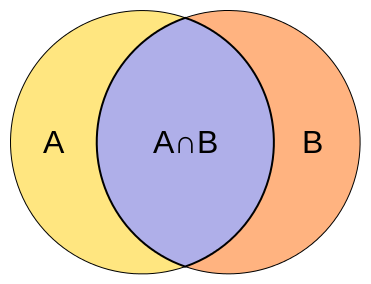
\includegraphics[width=0.45\textwidth]{images/Intersection_of_sets_A_and_B.png} 
        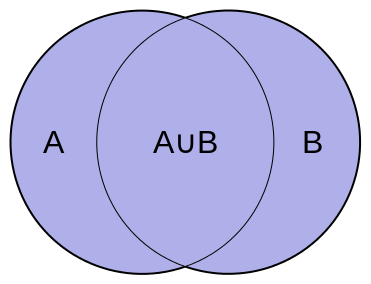
\includegraphics[width=0.45\textwidth]{images/Union_of_sets_A_and_B.png}
        \caption{Schnitt und Vereinigung of zweier Menge $ A $ and $ B $ \cite{intersectionImage,unionImage}}
    \end{figure}
\end{frame}


